\chapter{General Considerations of Electronic Transport}

%%%%%%%%%%%%%%%%%%%%%%%%%%%%
\section{Ohm's Law}
Ohm's law describes the relationship between the current ($I$) and applied voltage ($V$) or electric field ($E$) in a conductor and it can be expressed as \begin{equation} I = \frac{V}{R} 
\end{equation} where $R$ is the resistance and is a function of the size of conductor \begin{equation} R = \frac{\rho L}{A} = \frac{L}{A}\frac{1}{\sigma}
\end{equation} Hence, Ohm's law can be rewritten as \begin{equation}
I = \frac{V \sigma A}{L} \Rightarrow J = \frac{I}{A} = V \frac{\sigma}{L} = \sigma E
\end{equation} $\sigma$ is the conductivity and it's related to the mobility ($\mu = \frac{e \tau}{m^{*}}$). \begin{equation}
\sigma = ne\mu = \frac{e^{2} n \tau}{m^{*}}
\end{equation} From Equation (1.1) to (1.4), one may find that if $L$ is very small or $\tau$ (scattering or collision time) approaches to $\infty$ (happens when the temperature is close to zero), then the conductivity or current (density) would become huge without any bound. Therefore, the question is: What does the current look like in a very small device? The experimental result\footnote{Quantized Conductance of Point Contacts in a Two-Dimensional Electron Gas, B. J. van Wees et al., PRL, 1988} has shown that the conductance of a point contact is quantized at a low temperature, which seems to contradict Ohm's law shown above. Landauer's formula will be discussed in the next section to explore this issue.

%%%%%%%%%%%%%%%%%%%%%%%%%%%%%%%%%%%%%%
\section{Landauer's Formula}
Consider a device consisting of a hydrogen molecule (with two energy levels) connected between two contacts, as shown in Fig. 1.1. 
\begin{figure}[t]
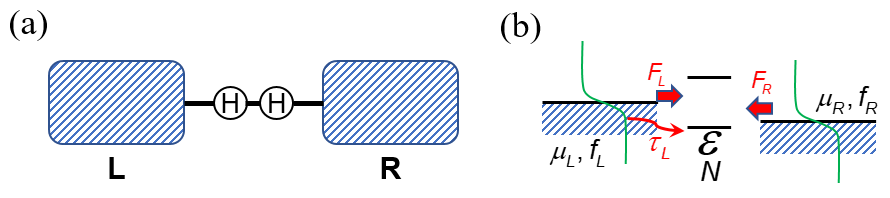
\includegraphics[width=\textwidth]{figures/Fig1_1}
\caption{\small (a) Schematic diagram of the "hydrogen molecule" device with left (L) and right (R) contact. (b) Energy diagram when applying a bias $-eV = \mu_{R}-\mu_{L}$. $F_{L,R}$ and $f_{L,R}$ are the electron flux and Fermi function of the left and right contacts. The green curves indicate the probability distribution of finding an electron (Fermi distribution).}
\end{figure}
We assume that when applying a bias $V$, the electrons can flow through the hydrogen molecule without scattering. Also, the Fermi function (distribution) is not applicable for the hydrogen molecule because the amount of electrons is not sufficient to be statistically meaningful\footnote{Ashley H. Carter, Classical and Statistical Thermodynamics.}. However, the contacts (like electron reservoirs) are assumed to be "large" enough to support the Fermi function. The equation of states (continuity equation) at a given energy $\varepsilon_i$ can be written as 
\begin{equation}
\frac{dN^{\varepsilon_i}}{dt} = F^{\varepsilon_i}_{L} + F^{\varepsilon_i}_{R}
\end{equation} 
where $N^{\epsilon_i}$ is the occupation factor at energy $\epsilon_i$ and the fluxes are 
\begin{equation}
F^{\varepsilon_i}_{L} = \frac{f^{\varepsilon_i}_{L}-N^{\varepsilon_i}}{\tau^{\varepsilon_i}_{L}}
\end{equation}
\begin{equation}
F^{\varepsilon_i}_{R} = \frac{f^{\varepsilon_i}_{R}-N^{\varepsilon_i}}{\tau^{\varepsilon_i}_{R}}
\end{equation} 
Hence, Equation (1.5) becomes\footnote{The superscript $\varepsilon_i$ is omitted for simplicity.} 
\begin{equation}
\frac{dN}{dt} + N \left(\frac{1}{\tau_{L}}+\frac{1}{\tau_{R}}\right) = \frac{f_{L}}{\tau_{L}}+\frac{f_{R}}{\tau_{R}}
\end{equation} 
Now, we define\footnote{The physical meaning will be discussed later.} 
\begin{equation}
\frac{1}{\tau_{L,R}} = \frac{\gamma_{L,R}}{\hbar}
\end{equation} where $\gamma$ has the unit of energy. Thus, we get 
\begin{equation}
\hbar \frac{dN}{dt} + N \left(\gamma_{L}+\gamma_{R}\right) = \gamma_{L} f_{L} + \gamma_{R} f_{R}
\end{equation} 
At steady state, we have 
\begin{equation}
N = \frac{\gamma_{L} f_{L} + \gamma_{R} f_{R}}{\gamma_{L}+\gamma_{R}}
\end{equation} 
Therefore, the current at energy $\varepsilon_i$ can be expressed as 
\begin{align}
I^{\varepsilon_i}&= e F^{\varepsilon_i}_{L} = e \frac{f^{\varepsilon_i}_{L}-N^{\varepsilon_i}}{\tau^{\varepsilon_i}_{L}}\nonumber\\
&=\frac{e}{\hbar} \gamma^{\varepsilon_i}_{L} \left(f^{\varepsilon_i}_{L}-\frac{\gamma^{\varepsilon_i}_{L} f^{\varepsilon_i}_{L} + \gamma^{\varepsilon_i}_{R} f^{\varepsilon_i}_{R}}{\gamma^{\varepsilon_i}_{L}+\gamma^{\varepsilon_i}_{R}}\right)\nonumber\\
&=\frac{e}{\hbar}\frac{\gamma^{\varepsilon_i}_{L}\gamma^{\varepsilon_i}_{R}}{\gamma^{\varepsilon_i}_{L}+\gamma^{\varepsilon_i}_{R}}\left(f^{\varepsilon_i}_{L}-f^{\varepsilon_i}_{R}\right)
\end{align} 
From Equation (1.12), one may directly observe that the current only depends on the properties of the contacts. Now if there are multiple energy levels, the current becomes
\begin{equation}
I = \sum_{\varepsilon_i} I^{\varepsilon_i} \times 2 = \sum_{\varepsilon_i}{\frac{e}{\hbar}\frac{\gamma^{\varepsilon_i}_{L}\gamma^{\varepsilon_i}_{R}}{\gamma^{\varepsilon_i}_{L}+\gamma^{\varepsilon_i}_{R}}\left(f^{\varepsilon_i}_{L}-f^{\varepsilon_i}_{R}\right)}\times2
\end{equation} 
where 2 is coming from the spin degeneracy. Use the following trick 
\begin{equation}
g\left(\varepsilon_i\right) = \int dE g\left(E\right) \delta\left(E-\varepsilon_i\right)
\end{equation} 
and Equation (1.13) can be rewritten as 
\begin{align}
I&= \int dE \left(\frac{2e}{\hbar}\right)\frac{\gamma^{E}_{L}\gamma^{E}_{R}}{\gamma^{E}_{L}+\gamma^{E}_{R}}\left(f^{E}_{L}-f^{E}_{R}\right)\sum_{\varepsilon_i}{\delta\left(E-\varepsilon_i \right)}\nonumber\\
&= \frac{2e}{\hbar}\int dE D\left(E\right) \frac{\gamma^E_{L}\gamma^E_{R}}{\gamma^E_{L}+\gamma^E_{R}} \left(f^E_{L}-f^E_{R}\right)
\end{align} 
where Equation (1.15) is {\bf Landauer's formula} and $D\left(E\right)$ is the density of states (DOS). 
\begin{equation}
D\left(E\right) = \sum_{\varepsilon_i}{\delta\left(E-\varepsilon_i\right)}
\end{equation} 
The general definition of DOS is the number of states per unit energy, so $D\left(E\right)$ also can be written as 
\begin{equation}
D\left(E\right) = \frac{\partial N^{CS}_{E}}{\partial E} = \lim_{\Delta E\rightarrow 0} \frac{N^{CS}_{E}\left(E+\Delta E\right)-N^{CS}_{E}\left(E\right)}{\Delta E}
\end{equation} 
where $N^{CS}_{E}$ is\footnote{Here is the cumulative sum (CS) of states at and below a given energy $E$.} 
\begin{equation}
N_{E}^{CS} = \sum_{\varepsilon_i}{\theta\left(E-\varepsilon_i\right)}
\end{equation} 
where $\theta\left(E-\varepsilon_i\right)$ is the Heaviside step function with the implicit degeneracy as shown in Fig. 1.2. For example, at energy $\varepsilon_{1}$ there are 5 states [Fig. 1.2(a)]. As it goes from low energy to high energy, the cumulative sum of states increases from 5 to 17 [Fig. 1.2(b)].
\begin{figure}[tbp]
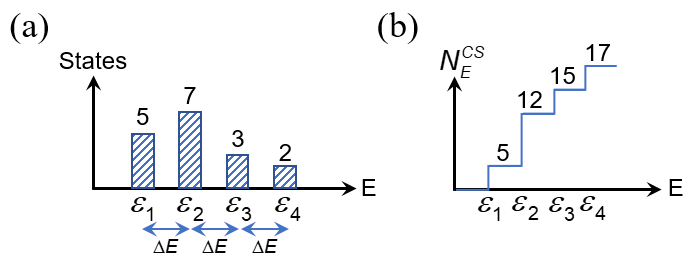
\includegraphics[width=0.7\textwidth]{figures/Fig1_2}
\centering
\caption{\small (a) Number of states distribution. (b) Cumulative sum of states.}
\end{figure} Thus, the Equation (1.17) becomes \begin{equation}
D\left(E\right) = \frac{\partial N^{CS}}{\partial E} = \sum_{\varepsilon_{i}}{\delta\left(E-\varepsilon_{i}\right)}
\end{equation} where $\delta\left(E-\varepsilon_{i}\right)$ is the delta function. After knowing the DOS, we obtain the total occupation factor $N$ 
\begin{align}
N&= \sum_{\varepsilon_{i}}{\frac{\gamma^{\varepsilon_i}_{L} f^{\varepsilon_i}_{L} + \gamma^{\varepsilon_i}_{R} f^{\varepsilon_i}_{R}}{\gamma^{\varepsilon_i}_{L}+\gamma^{\varepsilon_i}_{R}}}\nonumber\\
&= \int dE \frac{\gamma^E_{L} f^E_{L} + \gamma^E_{R} f^E_{R}}{\gamma^E_{L}+\gamma^E_{R}} \sum_{\varepsilon_{i}}{\delta\left(E-\varepsilon_{i}\right)}\nonumber\\
&= \int dE \frac{\gamma^E_{L} f^E_{L} + \gamma^E_{R} f^E_{R}}{\gamma^E_{L}+\gamma^E_{R}}D\left(E\right)
\end{align} 
Equation (1.20) is under the non-equilibrium condition. At the equilibrium condition (applied voltage $V = 0$), the Fermi functions and $\gamma$ of both contacts are the same ($f^E_{L} = f^E_{R} = f^E_{0}, \gamma^E_{L} = \gamma^E_{R}, \forall E$). Thus, the Equation (1.20) can be re-written as 
\begin{equation}
N = \int_{-\infty}^{\infty} D\left(E\right) f_{0}\left(E\right)dE
\end{equation} 
Equation (1.21) is commonly used to calculate the carrier concentration in semiconductors.\\
Now, we would like to figure out the maximum conductance based on Landauer's formula. Two assumptions are made in the following discussion: (1) the applied voltage $V$ is very small and (2) the temperature is fairly low. At small $V$, the Taylor expansion with the first two terms can be applied to the Fermi functions. 
\begin{equation}
    f_{L} = f_{0}\left(E-\mu_{L}\right)
\end{equation} 
\begin{align}
    f_{R}&= f_{0}\left(E-\mu_{R}\right)\nonumber\\
    &= f_{0}\left(E+eV-\mu_{L}\right)\nonumber\\
    &= f_{0}\left(E-\mu_{L}\right)+\left(\frac{\partial f_{0}}{\partial E}\right)eV
\end{align} 
Therefore, the Landauer's formula becomes 
\begin{align}
    I&= \frac{2e}{\hbar}\int dE D\left(E\right) \frac{\gamma^E_{L}\gamma^E_{R}}{\gamma^E_{L}+\gamma^E_{R}} \left(f^E_{L}-f^E_{R}\right)\nonumber\\
    &\approx \frac{2e^{2}}{\hbar}V\int dE D\left(E\right) \frac{\gamma^E_{L}\gamma^E_{R}}{\gamma^E_{L}+\gamma^E_{R}}\left(\frac{-\partial f_{0}}{\partial E}\right)
\end{align} 
Hence, the conductance $G$ is
\begin{equation}
    G = \frac{\partial I}{\partial V} = \frac{2e^{2}}{\hbar}\int dED\left(E\right) \frac{\gamma^E_{L}\gamma^E_{R}}{\gamma^E_{L}+\gamma^E_{R}}\left(\frac{-\partial f_{0}}{\partial E}\right)
\end{equation} 
When the temperature approaches zero, the derivative of the Fermi function with respect to the energy $E$ is like a delta function (see Fig. 1.3) 
\begin{figure}[tbp]
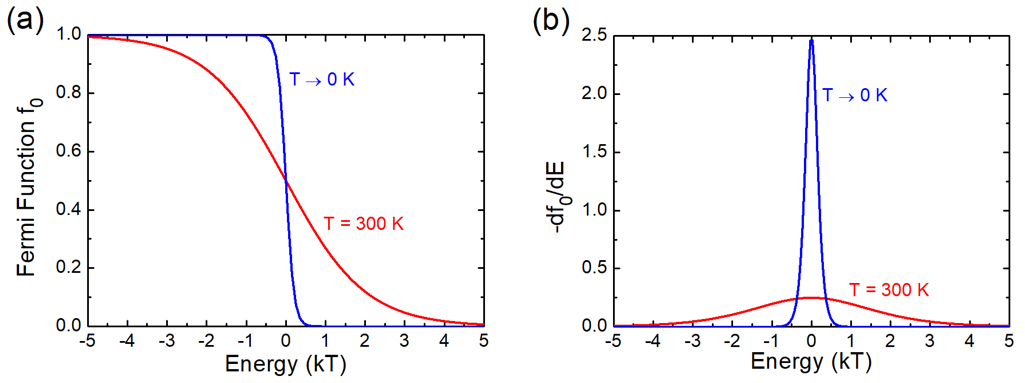
\includegraphics[width=0.9\textwidth]{figures/Fig1_3}
\centering
\caption{\small (a) Fermi functions and (b) their derivative at different temperatures. The Fermi level is located at $E = 0$.}
\end{figure}
\begin{equation}
    \left(\frac{-\partial f_{0}\left(E - \mu_L \right)}{\partial E}\right) \rightarrow \delta\left(E-\mu_{L}\right)
\end{equation} and the conductance $G$ becomes 
\begin{align}
    G& = \frac{2e^{2}}{\hbar}\int dE D\left(E\right) \frac{\gamma^E_{L}\gamma^E_{R}}{\gamma^E_{L}+\gamma^E_{R}}\delta\left(E-\mu_{L}\right)\nonumber\\
    &= \frac{2e^{2}}{\hbar}\left[D\left(E\right)\frac{\gamma^E_{L}\gamma^E_{R}}{\gamma^E_{L}+\gamma^E_{R}}\right]_{E = \mu_L}
\end{align} 
To further examine the Equation (1.27), the concept of "energy broadening" should be introduced.

%%%%%%%%%%%%%%%%%%%%%%%%%%%%%%%%%%%%%%%%%%%%%%%%%
\section{Broadening and Maximum Conductance}
Due to the wave nature of the quantum objects, the uncertainty principle is inherent in the system we discussed. The uncertainty principle states that complementary variables, such as position/momentum and energy/time, cannot be measured simultaneously\footnote{D. J. Griffiths, Introduction to Quantum Mechanics, Chapter 3.}. 
\begin{equation}
    \Delta E \Delta t \geq \frac{\hbar}{2}
\end{equation} 
The $\Delta t$ can be interpreted as the ``lifetime" of electrons, implying that the $\Delta E$ is non-zero, which is called energy ``broadening." This effect has been seen in Equation (1.9) where $\gamma$ is interpreted as the energy broadening. When the atomistic device interacts with a large quantum system (L and R contacts), the energy levels no longer remain discrete but change to a spectrum-like distribution (broadening). However, the shape of the energy broadening is difficult to be experimentally determined, so we utilize the Lorentzian equation\footnote{We would like a function with (1) symmetry and (2) area under the curve $=1$.} to get analytic results \begin{equation}
    \delta\left(E-\varepsilon_{i}\right) \xrightarrow{\text{Broadening}} \frac{1}{2\pi}\frac{\gamma_{L}+\gamma_{R}}{\left(E-\varepsilon_{i}\right)^{2}+\left(\frac{\gamma_{L}+\gamma_{R}}{2}\right)^{2}}
\end{equation} 
For the Lorentzian equation, $\gamma_{L/R}$ are constants and not a function of energy. Then Equation (1.29) gives 
\begin{equation}
    \int_{-\infty}^{\infty} dE \frac{1}{2\pi}\frac{\gamma_{L}+\gamma_{R}}{\left(E-\varepsilon_{i}\right)^{2}+\left(\frac{\gamma_{L}+\gamma_{R}}{2}\right)^{2}} = \frac{\gamma_{L}+\gamma_{R}}{2\pi}\frac{2}{\gamma_{L}+\gamma_{R}}\arctan\left({\frac{E-\varepsilon_{i}}{\frac{\gamma_{L}+\gamma_{R}}{2}}}\right)\bigg|_{-\infty}^{\infty}=1
\end{equation} 
Therefore, the Equation (1.27) can be re-written as 
\begin{align}
    G& = \frac{2e^{2}}{\hbar}\sum_{\varepsilon_{i}}{\delta\left(E-\varepsilon_{i}\right)} \frac{\gamma^E_{L}\gamma^E_{R}}{\gamma^E_{L}+\gamma^E_{R}}\bigg|_{E=\mu_{L}}\nonumber\\
    &\xrightarrow{\text{Broadening}} \frac{2e^{2}}{\hbar}\sum_{\varepsilon_{i}}{\frac{1}{2\pi}\frac{\gamma_{L}+\gamma_{R}}{\left(\mu_{L}-\varepsilon_{i}\right)^{2}+\left(\frac{\gamma_{L}+\gamma_{R}}{2}\right)^{2}}} \frac{\gamma_{L}\gamma_{R}}{\gamma_{L}+\gamma_{R}}\nonumber\\
    &= \frac{2e^{2}}{h}\sum_{\varepsilon_{i}}{\frac{4\gamma_{L}\gamma_{R}}{4\left(\mu_{L}-\varepsilon_{i}\right)^{2}+\left(\gamma_{L}+\gamma_{R}\right)^{2}}}\nonumber\\
    &\xrightarrow[\mu_{L}=\varepsilon_{i}]{maximum} \frac{2e^{2}}{h}{\frac{4\gamma_{L}\gamma_{R}}{\left(\gamma_{L}+\gamma_{R}\right)^{2}}M}
\end{align} 
M is the number of degenerate states at energy $\varepsilon_i$ called the number of modes. From the inequality of arithmetic and geometric means\footnote{$\frac{a+b}{2}\geq\sqrt{ab}\Rightarrow\frac{4ab}{\left(a+b\right)^{2}}\leq1$}, the maximum conductance is \begin{equation}
    G^{max} = \frac{2e^{2}}{h}M
\end{equation} 
Equation (1.32) indicates that the material band structure and dimensionality limit the maximum conductance. This is also why plateaus are observed in the conductance measurement at low temperatures.

%%%%%%%%%%%%%%%%%%%%%%%%%%%%%%%%%%%%%%%%%%%%%%%
\section{Electrostatics}
In the previous sections, the device with two terminals is discussed. Now, let's consider a three-terminal device (like MOSFET) with an insulator layer and a gate contact on the top of the channel as shown in Fig. 1.4.
\begin{figure}[tbp]
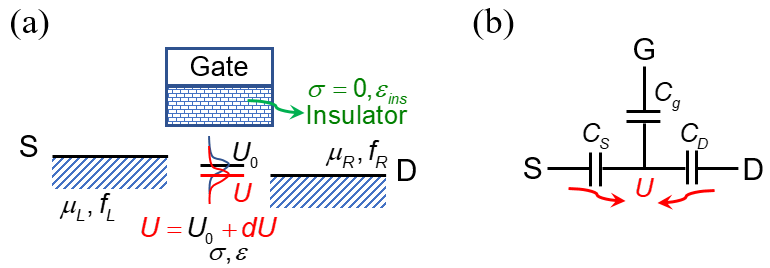
\includegraphics[width=0.8\textwidth]{figures/Fig1_4}
\centering
\caption{\small (a) Schematic diagram of the gated device. The energy level in the channel is broadened due to the current flow. (b) The equivalent circuit of the gated device. $U$ and $U_{0}$ are the energy with and without biases.}
\end{figure} When the gate voltage is applied ($V_{g} \neq 0, V_{S} = V_{D} = 0$), the energy level in the channel is pulled down due to more electrons induced and the change in the electrostatic potential ($\phi$) in the channel can be expressed as 
\begin{equation}
    d\phi = \frac{C_{g}}{C_{g}+C_{S}+C_{D}}dV_{g}
\end{equation}
and the occupation factor with ($N$) and without bias ($N_{0}$)  are \begin{equation}
    N = \int_{-\infty}^{\infty} dE \frac{\gamma_{L} f_{L} + \gamma_{R} f_{R}}{\gamma_{L}+\gamma_{R}}D\left(E-U\right)
\end{equation}
\begin{equation}
    N_{0} = \int_{-\infty}^{\infty} dE \frac{\gamma_{L} f_{L} + \gamma_{R} f_{R}}{\gamma_{L}+\gamma_{R}}D\left(E-U_{0}\right)
\end{equation}
\begin{equation}
    \delta N \equiv N - N_{0}
\end{equation} Similarly, if $V_{S} \neq 0, V_{g} = V_{D} = 0$, the potential change is \begin{equation}
    d\phi = \frac{C_{S}}{C_{g}+C_{S}+C_{D}}dV_{S}
\end{equation} and if $V_{D} \neq 0, V_{g} = V_{S} = 0$, \begin{equation}
    d\phi = \frac{C_{D}}{C_{g}+C_{S}+C_{D}}dV_{D}
\end{equation} Finally, if $V_{g} = V_{S} = V_{D} = 0$, and $Q$ is the amount of charge present in the channel, 
\begin{equation}
    d\phi = \frac{dQ}{C_{g}+C_{S}+C_{D}}
\end{equation} Combining above equations, we obtain \begin{equation}
    d\phi = \alpha_{g} dV_{g} + \alpha_{D} dV_{D} + \alpha_{S} dV_{S} + \frac{dQ}{C_{g}+C_{S}+C_{D}}
\end{equation} where \begin{equation}
    \alpha_{g,S,D} = \frac{C_{g,S,D}}{C_{g}+C_{S}+C_{D}}
\end{equation} The Equation (1.40) also can be expressed using energy $U$ (Multiplying $-e$ to the above equation) 
\begin{align}
    dU& = \alpha_{g} U_{g} + \alpha_{D} U_{D} + \alpha_{S} U_{S} - \frac{edQ}{C_{g}+C_{S}+C_{D}}\nonumber\\
    & = \alpha_{g} U_{g} + \alpha_{D} U_{D} + \alpha_{S} U_{S} + \frac{e^{2}\delta N}{C_{g}+C_{S}+C_{D}}
\end{align} The Equation (1.42) tells us that when increasing the number of electrons (occupation) in the channel, there is an energy penalty that resists the changes. Solving Equation (1.34), (1.35), (1.36), and (1.42) by iterations, the energy $U$ is obtained and the current can be immediately calculated using Landauer's formula \begin{equation}
    I = \frac{2e}{\hbar}\int dE D\left(E-U\right) \frac{\gamma_{L}\gamma_{R}}{\gamma_{L}+\gamma_{R}} \left(f_{L}-f_{R}\right)
\end{equation} where we define 
\begin{equation}
    D\left(E-U\right) \frac{\gamma_{L}\gamma_{R}}{\gamma_{L}+\gamma_{R}} \equiv T\left(E\right)
\end{equation} is the transmission probability due to scatterings. Assuming the applied drain-to-source voltage ($V$) is small and the energy broadening follows Equation (1.29), we have 
\begin{align}
    I& = \frac{2e}{\hbar}\sum_{\varepsilon_{i}}{\int dE \frac{1}{2\pi}\frac{\gamma_{L}+\gamma_{R}}{\left(E-\varepsilon_{i}\right)^{2}+\left(\frac{\gamma_{L}+\gamma_{R}}{2}\right)^{2}} \frac{\gamma_{L}\gamma_{R}}{\gamma_{L}+\gamma_{R}} \left(\frac{-\partial f_{0}}{\partial E}\right)eV}\nonumber\\
    &= \frac{2e^2}{h}V\sum_{\varepsilon_{i}}{\underbrace{\int dE\times \frac{\gamma_{L}\gamma_{R}}{\left(E-\varepsilon_{i}\right)^{2}+\left(\frac{\gamma_{L}+\gamma_{R}}{2}\right)^{2}} \left(\frac{-\partial f_{0}}{\partial E}\right)}_{\equiv \overline{T}_{}\varepsilon_{i}}}\nonumber\\
    &= \frac{2e^{2}}{h}V\overline{M}\cdot\overline{T}_{\varepsilon_{i}}
\end{align} where $\overline{M}$ is the average number of modes around the Fermi energy. The resistance is \begin{equation}
    R = \frac{\partial V}{\partial I} = \frac{h}{2e^{2}\overline{M}}\cdot\frac{1}{\overline{T}_{\varepsilon_{i}}}
\end{equation} 

Changes made by student and checking action workflow
